\documentclass{sebaClass}
\usepackage{float}
\usepackage{bm}
\usepackage{siunitx}

\title{Projet}
\author{Ying, Philippe et Sébastien}
\date{30 novembre 2021}

\newcommand{\SubTitle}{Projet systèmes concurrents/intergiciels}
\newcommand{\Subject}{Linda}
\newcommand{\Place}{ENSEEIHT}

\renewcommand{\Language}{text}
\newcommand{\cFF}[3]{\codeFromFile{text}{#1}{#2}{#3}}
\newcommand{\cFFS}[1]{\codeFromFileSimple{text}{#1}}
\newcommand{\cFFSC}[1]{\codeFromFileSimpleContinuousLine{text}{#1}}
\newcommand{\sFF}[3]{\shellFromFile{#1}{#2}{#3}}
\newcommand{\q}[1]{\textit{\textbf{#1}}\\}
\newcommand{\ql}[1]{\textit{\textbf{#1}}}
\newcommand{\rt}[1]{\textcolor{redl}{#1}}

\begin{document}

\maketitle
\tableofcontents
% \listoffigures

\vspace*{\fill}
\textit{\underline{Remarque :} Ceci est le document réponse, il ne reprend pas l'intégralité du sujet.}
\newpage

\section{Introduction}
\subsection{Membres de groupe}

Nous sommes trois étudiants du groupe M2 :
\begin{dinglist}{111}
    \item Ying LIU
    \item Philippe NEGREL-JERZY
    \item Sébastien PONT
\end{dinglist}

\subsection{Présentation}

Nous ne représentons pas tout le sujet (que vous pouvez retrouver \href{https://spont.me/mjxoog}{ici}\footnote{\href{https://spont.me/mjxoog}{https://spont.me/mjxoog}}), mais voici un résumé.

Linda est un service permettant de partager des données sous formes de \iCode{Tuple}.
Dans ce projet nous allons implémenter deux manières de partager et gérer ces ressources à travers plusieurs clients :

\begin{itemize}
    \item une version dite "locale" à base de mémoire partagée (\iCode{shm} package Figure \ref{fig:main_class_diagram})
    \item une version dite "distante" à base de clients / monoserveur (\iCode{server} package Figure \ref{fig:main_class_diagram})
\end{itemize}

\begin{figure}[H]
    \centering
    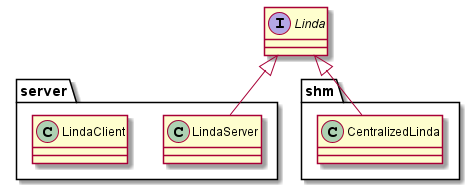
\includegraphics[scale=0.7]{src/part-01/mainCD.png}
    \caption{Diagramme de classe général du projet} \label{fig:main_class_diagram}
\end{figure}

\begin{dinglist}{111}
    \item Version mémoire partagée (version locale) :
    \item
    \item Version client / monoserveur (version distante)
\end{dinglist}

\end{document}